\documentclass[10pt, a4paper,spanish]{article}

\usepackage[utf8]{inputenc}
\usepackage[spanish]{babel}

\usepackage[T1]{fontenc}

\usepackage[hmarginratio=1:1,top=32mm,columnsep=20pt]{geometry}
\usepackage[hang, small,labelfont=bf,up,textfont=it,up]{caption}


\usepackage{graphicx}
\graphicspath{ {images/} }

\usepackage{titlesec}
\renewcommand\thesection{\Roman{section}}
\renewcommand\thesubsection{\Roman{subsection}}
\titleformat{\section}[block]{\large\scshape\centering}{\thesection.}{1em}{}
\titleformat{\subsection}[block]{\large}{\thesubsection.}{1em}{}

\usepackage{fancyhdr}
\pagestyle{fancy}
\fancyhead{}
\fancyfoot{}
\fancyhead[C]{ \today \ $\bullet$ Minería de Datos $\bullet$ Lógica y Representación del Conocimiento}
\fancyfoot[RO]{\thepage}

%-------------------------------------------------------------------------------
%	TITLE SECTION
%-------------------------------------------------------------------------------

\title{\vspace{-15mm}\fontsize{24pt}{10pt}\selectfont\textbf{Lógica y Representación del Conocimiento}} % Article title

\author{Sergio García Prado}
\date{\today}

%-------------------------------------------------------------------------------

\begin{document}

	\maketitle % Insert title

	\thispagestyle{fancy} % All pages have headers and footers

%-------------------------------------------------------------------------------
%	TEXT
%-------------------------------------------------------------------------------

	\begin{center}
		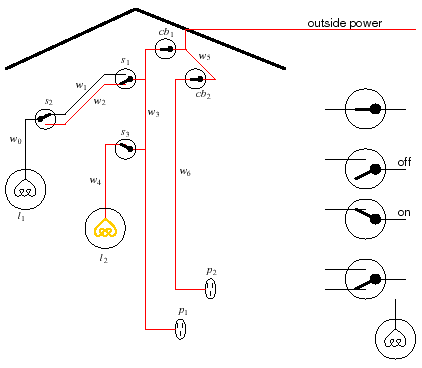
\includegraphics[width=0.6\textwidth]{diagnostic-assistant}
	\end{center}

	\section{Elaborar una base de conocimiento para el asistente al diagnóstico en el dominio del cableado de una vivienda. Las reglas generales deben de permitir codificar la instancia específica que muestra la figura. Utilizar los principios generales para la elaboración de una ontología específica.}


		\paragraph{}
		Vocabulario: \\

		\paragraph{}
		Constantes: \\
		%
		$On$ \\
		$Off$ \\
		%
		$Up$ \\
		$Down$ \\
		%
		$CircuitBreaker$ \\
		$Switch$ \\
		$Light$ \\
		$PowerOutlet$ \\
		$Wire$ \\
		%
		$CB_i, i \in \{1,2\}$ \\
		$S_i \in \{1,2,3\}$ \\
		$L_i \in \{1,2\}$ \\
		$PO_i \in \{1,2\}$ \\
		$W_i \in \{1,2,3,4,5,6\}$ \\
		$OutsidePower$ \\

		\paragraph{}
		Predicados:

		\begin{itemize}
			\item $Light(x) \equiv$ La variable $x$ luce.
			\item $Electrize(x) \equiv$ La variable $x$ produce electricidad (para enchufes).
			\item $Ok(x) \equiv$ La variable $x$ presenta un funcionamiento correcto.
			\item $Connected(x, y) \equiv$ La variable $x$ está conectada a la variable $y$.
		\end{itemize}


		\paragraph{}
		Funciones:
		\begin{itemize}
			\item $in(x) = y \equiv$ La entrada de $x$ es $y$.
			\item $out(x,y) = z \equiv$ La salida $y$ de $x$ es  $z$.
			\item $signal(x) = y \equiv$ La señal de $x$ es  $y $.
			\item $state(x) = y \equiv$ El estado de $x$ es $y$.
			\item $type(x) = y \equiv$ El tipo de $x$ es $y$.
		\end{itemize}




		\paragraph{}
		Ontología general:
		\begin{itemize}

			%types
			\item Restricciones de Tipos de Componentes
			\begin{itemize}
				\item $ CircuitBreaker \neq Switch\neq Ligth \neq PowerOutlet \neq Wire   $
				\item $ \forall x [((type(x) = CircuitBreaker) \lor (type(x) = Switch) \lor (type(x) = Ligth) \lor (type(x) = PowerOutlet) \lor (type(x) = Wire))] $
			\end{itemize}
			% Connections
			\item Restricciones de Conexiones.
			\begin{itemize}
				\item $ On \neq Off $
				\item $ \forall x [((signal(x) = On) \lor (signal(x) = Off))] $
				\item $ \forall x \forall y [(Connected(x, y) \supset Connected(y, x))] $
				\item $ \forall x \forall y [(Connected(x, y) \land Ok(x) \land Ok(y) \supset (signal(x) = signal(y)))] $
			\end{itemize}

			% Switchess
			\item Restricciones de Conmutadores.
			\begin{itemize}
				\item $ Up \neq Down $
				\item $ \forall x [((state(x) = Up) \lor (state(x) = Down))] $
				\item $ \forall x [( (type(x) = Switch) \supset ((state(x) = Up) \lor (state(x) = Down)))] $
				\item $ \forall x [( ( (type(x) = Switch) \land (state(x) = Up) ) \supset Connected(in(x), out(x, Up)))] $
				\item $ \forall x [( ( (type(x) = Switch) \land (state(x) = Down) ) \supset Connected(in(x), out(x, Down)))] $
			\end{itemize}

			% Circuit Breakers
			\item Restricciones de diferenciales.
			\begin{itemize}
				\item $ \forall x \forall y \forall z [( ((type(y) = CircuitBreaker) \land Connected(x, y) \land Connected(y, z) ) \supset Connected(x, z))] $
			\end{itemize}

			% Lights
			\item Restricciones de Bombillas.
			\begin{itemize}
				\item$ \forall x [(((signal(x) = On) \land (type(x) = Light) )  \supset Light(x))] $
			\end{itemize}

			% Power Outlets
			\item Restricciones de Enchufes.
			\begin{itemize}
				\item$ \forall x [(((signal(x) = On) \land (type(x) = PowerOutlet) )  \supset Electrize(x))] $
			\end{itemize}
		\end{itemize}




		\paragraph{}
		Ontología específica:



	\section{Partiendo de la base de conocimiento del asistente al diagnóstico que hemos utilizado en las prácticas de la asignatura, elaborar la ontología que la soporta. Compararla con la ontología elaborada en el problema anterior.}

		\paragraph{}



\end{document}
